В данном разделе представлен обзор и анализ различных задач для автоматизации с зависимостью от времени, а также аналогов реле времени РВ-90. В конце раздела составлен краткий обзор достоинств и недостатков реле времени с выводами.


\subsection{Область применения}
Автоматизация с зависимостью от времени может быть востребована во многих  ситуациях. Далее исследуются возможные применения реле времени в разных областях.

\subsubsection{Городское хозяйство}
В любом крупном городе освещение улиц и фасадов контролируется с точностью до минуты в соответствии с ежегодным календарем, утвержденным администрацией города. Отдельные архитектурные и исторические объекты, а также памятники обычно имеют свои утвержденные годовые графики подсветки[2]. И график включения/выключения отличается от уличного и должен быть введен в действие отдельно. В целях экономии электроэнергии световая реклама, подсветки вывесок магазинов и кафе переключается в ночной режим вечером и возвращается в дневной режим утром. В школах и других  учебных заведениях используют звонки, чтобы сигнализировать о начале или конце урока и перемены.


\subsubsection{Сельское хозяйство}
В сельском хозяйстве посевы необходимо поливать по определенному расписанию. Этот график отличается в зависимости от сорта растений. Для газонов используется отдельный график полива[3]. В теплицах по суточному графику может осуществляется подсветка растений. На птицефабриках подсветка и кормление также осуществляется по часам.


\subsubsection{Производство}
Заводы должны ежедневно включать кондиционер и отопление в рабочее время суток и выключать их в ночное время, автоматизация этого процесса еще больше осложняется тем, что время включения/выключения для таких систем различно в выходные, праздничные и сокращенные дни[4]. 


\subsection{Существующие решения}
На текущий момент на низком и среднем ценовых сегментах рынка существуют несколько типов устройств для автоматизации изложенных выше задач. Их можно разделить на две категории: механические реле и электронные реле.

\subsubsection{Механические реле}
Механические реле времени имеют простое внутреннее устройство. Механический диск вращается с периодом 24 часа и с помощью мелких дип-переключателей на диске можно задать время включения и выключения. Эти реле предельно просты в эксплуатации, однако недостатком является то, что в таком формате можно реализовать только суточные реле с циклом который повторяется каждые 24 часа (невозможно задать программу на 2 дня, на неделю, на год). И, также, проблема в том, что число включений и выключений ограничено количеством дип-переключателей на диске, и, как правило, наименьший промежуток времени между включением и выключением другими словами точность срабатывания реле, составляет 15 минут. Механические реле не имеют никакого программного обеспечения.

Многие известные производители электротехники выпускают подобные устройства[5]. 
Западные производители: ABB[6], Siemens[7], Legrand, Orbis, Еuroautomatica, Elko
Китайские производители: Chint, IEK и д.р.

Реле времени 2РВМ (рис 1.) является типичным реле с анкерным механизмом. Оно предназначено для управления двумя независимыми электрическими цепями на замыкание или размыкание[8].

\begin{figure}[h!]
    \centering
    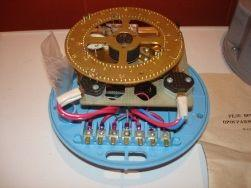
\includegraphics[width=0.5\textwidth]{mechanical_rele.png}
    \caption{Реле времени 2РВМ}
\end{figure}


\textbf{Преимущества}
\begin{my_enumerate}
\item Предельно просты в эксплуатации.
\item Надежны в работе.
\end{my_enumerate}

\textbf{Недостатки}
\begin{my_enumerate}
\item Программа только на 24 часа (нельзя задать программу на 2 дня, на год).
\item Число включений/выключений ограничено количеством дип-переключателей на диске.
\item Точность выбора времени включения/выключения - кратное 15 минут.
\end{my_enumerate}


\subsubsection{Электронные реле}
Наиболее распространенный тип реле времени, в основе которого используется микроконтроллер исполняющий загруженное в него программное обеспечение. Имеют различные входы и выходы для осуществления обратной связи, развитое программирование для задания необходимого алгоритма включений/выключений.  Поскольку в таких устройствах может использоваться кварцевая стабилизация частоты то они обеспечивают очень высокую точность[9]. В электронных реле можно задать программу работы на сутки, неделю и даже несколько лет. Можно выбрать время включения и выключения с высокой точностью до секунды, а количество событий включений и отключений которые можно запрограммировать в память реле измеряется сотнями. 

\subsubsection*{Реле на основе микроконтроллера}

Устройство которое использует LCD экран и кнопки управления для предоставления пользователю возможностей настройки.
Пример устройства РЭВ-302 (Новатэк-электро, Одесса, Украина) показан на рисунке 2.

\begin{figure}[h!]
    \centering
    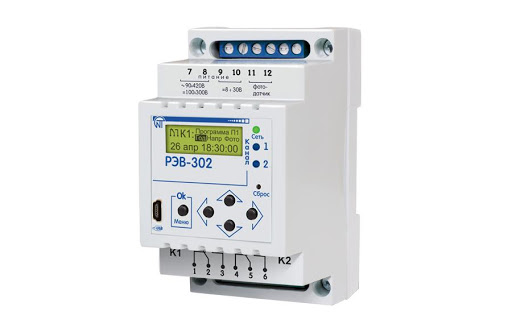
\includegraphics[width=0.5\textwidth]{rev302.png}
    \caption{Прибор РЭВ-302}
\end{figure}


РЭВ-302 можно настроить для включения и выключения периферийного прибора, например бойлера, в загородном доме в зависимости от точной даты и времени. Однако РЭВ-302 и аналоги излишне сложны в настройке.  Маленький LCD экран серьезно ограничивает возможность вывода полезной информации пользователю. Для настройки, навигации по меню, а также для ввода всех числовых значений имеются лишь несколько кнопок на передней панели, что делает процесс медленным и подверженным ошибкам. Устройство не предоставляет опции из коробки для удаленной работы. Получить обзор текущей конфигурации также очень сложно, что затрудняет работы по техническому обслуживанию и поддержке. Наконец, пользователь должен быть хорошо знаком с объемной инструкцией к изделию, для того чтобы успешно перемещаться по меню параметров и конфигурации. 

Реле времени РЭВ-302 выделяется тем что имеет micro-USB порт и поддерживает технологию USB-OTG. Таким образом данное реле можно настраивать с компьютера или с телефона/планшета[10]. Однако есть серьезные ограничения с поддержкой различных конфигураций операционных систем и платформ.

При настройки с ПК требуется наличие строго ОС Windows, а также наличие специальной программы для Windows от Новатэк-электро. При настройке с телефона/планшета требуется наличие строго ОС Android, а также наличие специального приложения для Android от Новатэк-электро. Любые другие конфигурации операционных систем и платформ не поддерживаются.

\textbf{Преимущества}
\begin{my_enumerate}
\item Можно задать программу работы на сутки, на неделю или на год.
\item Точность выбора времени включения/выключения - кратное секунде
\item Очень большое количество событий для включений и отключений.
\end{my_enumerate}

\textbf{Недостатки}
\begin{my_enumerate}
\item Маленький экран.
\item Объемная инструкция.
\item Очень неудобно программировать.
\item Затруднены работы по техническому обслуживанию и поддержке, если надо что-либо проверить/поменять в настройках.
\item Высокая цена
\end{my_enumerate}


\subsubsection*{Реле на основе микроконтроллера со встроенным модулем Wi-Fi}

Устройство которое использует сети Wi-Fi для предоставления пользователю возможности удаленной настройки и удобного интерфейса. 

Наиболее схожим с РВ-90 является линейка изделий Sonoff (Айтихэд Интеллектуальные Системы, Шэньчжэнь, Китай). Это очень бюджетные реле времени которые могут быть сопряжены со смартфоном посредством приложения eWeLink доступного на мобильных платформах. 

Однако у них есть и некоторые существенные недостатки. Во-первых, настройка реле происходит только через мобильное приложение eWeLink, из за чего данное реле невозможно настроить через ПК. Во-вторых, устройства Sonoff требуют подключения к интернету поскольку взаимодействие между пользователем и реле осуществляется через облачный сервер. Это может приводить к задержкам и сбоям в срабатывании реле.  Доступ к сети интернет делает их уязвимыми для атак.  Этот факт особенно важен учитывая что в устройствах Sonoff был обнаружен ряд серьезных уязвимостей, позволяющих используя механизм обновления по воздуху (OTA) обновить или полностью заменить заводскую прошивку реле без ведома или одобрения владельца. Также известно что устройства Sonoff не проверяли SSL-сертификаты на достоверность хотя они использовали HTTPS[11] соединение. Данного рода уязвимости позволяют проводить атаки направленные на перехват или манипуляцию команд обмениваемых между пользователем и устройством.

\textbf{Преимущества}
\begin{my_enumerate}
\item Можно контролировать удаленно
\item Точность выбора времени включения/выключения - кратное секунде
\item Достаточно большое количество событий для включений и отключений.
\item Невысокая цена
\end{my_enumerate}

\textbf{Недостатки}
\begin{my_enumerate}
\item Необходим доступ в интернет
\item Зависимость от облачных сервисов
\item Нет возможности настроить с ПК, только из приложения eWeLink
\item Проблемы с безопасной передачей данных через интернет
\end{my_enumerate}


\filbreak
\subsection{Определение характеристик желаемого решения}

Рассмотрев различные реле времени, можно составить краткий обзор достоинств и недостатков электронных реле времени, а также выделить важные характеристики которые будут важны при проектировании архитектуры системы.


При планировании архитектуры программы для управления и взаимодействия с реле времени РВ-90 следует учесть следующие требования:
\begin{my_itemize}
\item Безопасность и стабильность работы системы первостепенны.
\item Программа должна иметь максимально простой и интуитивный интерфейс. Т.к. механические реле все еще используются именно из-за их простоты в настройке.
\item Программа должна предоставлять возможность настройки с экрана ПК или мобильного телефона.  
\item Необходима поддержка различных конфигураций операционных систем и платформ. Нет смысла поддерживать только одну из многих платформ.
\item Программа не должна быть зависимым от облачного сервера.
\item Для снижения цены изделия отлично подойдет микроконтроллер со встроенной периферией Wi-Fi.
\item Программа должна поддерживать большое количество событий включений/выключений с точностью до секунды.
\end{my_itemize}


\subsection{Выводы по главе}
Для более глубокого понимания специфики индустрии были рассмотрены процессы которые могут быть автоматизированы с помощью реле времени. Помимо этого были рассмотрены наиболее часто применяемые изделия вместе с их сильными и слабыми сторонами. В результате пополнен состав требований к программе.






